\chapter{Resumen}

La aplicación desarrollada para este Trabajo de Fin de Máster consiste en un software modular programado en Python que se ejecuta desde la terminal de comandos. Su función principal es automatizar la extracción de texto y la comprensión visual de páginas en formato PDF pertenecientes a gramáticas de lenguas mayas. El sistema inyecta ejemplos estructurados de entrada y salida (few-shot) junto a un prompt especializado directamente en la memoria de la API de Gemini, logrando que el modelo de Inteligencia Artificial entienda la disposición tipográfica original y devuelva la información totalmente organizada en un archivo XML con etiquetas semánticas personalizadas (como <morpheme\_analysis> o <syntactic\_analysis>). Posteriormente, el pipeline procesa este archivo XML para generar de forma automática un documento en LaTeX que se compila para reconstruir la obra original en un nuevo archivo PDF con un acabado editorial profesional. El objetivo último es transformar "papel digital" estático en un conjunto de datos estructurados de alta precisión (Gold Standard) que sirva como combustible indispensable para que, en el futuro, otras Inteligencias Artificiales puedan entrenarse y aprender idiomas minorizados de bajos recursos computacionales.
Este Trabajo de Fin de Máster aborda la problemática de la digitalización y estructuración de gramáticas normativas de lenguas mayas minorizadas (Kaqchikel, K’iche’, Mam y Q’anjob’al), cuyos documentos originales presentan estructuras tipográficas complejas que dificultan el procesamiento mediante técnicas de OCR convencionales. Se propone y desarrolla un sistema automatizado basado en Modelos de Lenguaje de Gran Tamaño (LLMs) a través de la API de Gemini, integrado en un pipeline modular desarrollado en Python. Con este flujo se consigue mitigar la pérdida de información semántica y espacial inherente a los métodos planos tradicionales, salvaguardando recursos científicos de alto valor como las glosas interlineales.
La metodología se fundamenta en la transformación de documentos PDF en datos estructurados bajo el estándar XML, garantizando la integridad jerárquica mediante la definición de un Documento de Definición de Tipo (DTD) y el desarrollo de módulos específicos de corrección estructural (xml\_corrector.py). El núcleo de la investigación se centra en un estudio empírico sobre el parámetro de temperatura del modelo, evaluando su impacto en la precisión y estabilidad del sistema bajo una estricta "economía de tokens" impuesta por las limitaciones de cuota del entorno operativo.
Los resultados experimentales demuestran la existencia de un "punto dulce" (sweet spot) en temperaturas de 0.1 y 0.25, donde se alcanzan precisiones superiores al 90% incluso en casos de alta complejidad estructural y estrés informativo. Finalmente, el sistema automatiza la generación de documentación científica en LaTeX, permitiendo una reconstrucción fiel y profesional de los textos originales. El trabajo concluye que el uso de LLMs, correctamente parametrizados y validados mediante un entorno de control heurístico y formal, constituye una herramienta de alto valor para la preservación del patrimonio lingüístico digital y la soberanía tecnológica de las comunidades desfavorecidas.


\textbf{Palabras clave:} Inteligencia Artificial, LLM, Gemini API, Lenguas Mayas, Digitalización, XML, Procesamiento de Lenguaje Natural, OCR Estructurado.


\chapter*{Motivación y justificación}
\thispagestyle{empty}

La preservación de la diversidad lingüística constituye uno de los desafíos más críticos en la era de la información. Las lenguas minorizadas, en particular aquellas pertenecientes a la familia maya como el Kaqchikel, el K’iche’, el Mam y el Q’anjob’al, representan un patrimonio cultural de valor incalculable. Sin embargo, su supervivencia no sólo depende de su uso oral, sino también de la disponibilidad y accesibilidad de recursos académicos y normativos en formatos digitales modernos.
En este contexto, la Academia de Lenguas Mayas de Guatemala (ALMG) desempeña un papel crucial como entidad rectora en la promoción y estandarización de estos idiomas. A través de su repositorio institucional de documentos (disponible en https://almg.org.gt/documentos/), la ALMG ha realizado un esfuerzo significativo por poner a disposición del público gramáticas normativas y textos de referencia, tal y como se muestra en la figura \ref{fig:web_ALMG}. No obstante, gran parte de este conocimiento se encuentra consignado en archivos PDF que, si bien facilitan la difusión, actúan esencialmente como "papel digital": una representación estática de la información que carece de estructura semántica.


\begin{figure}
    \centering
    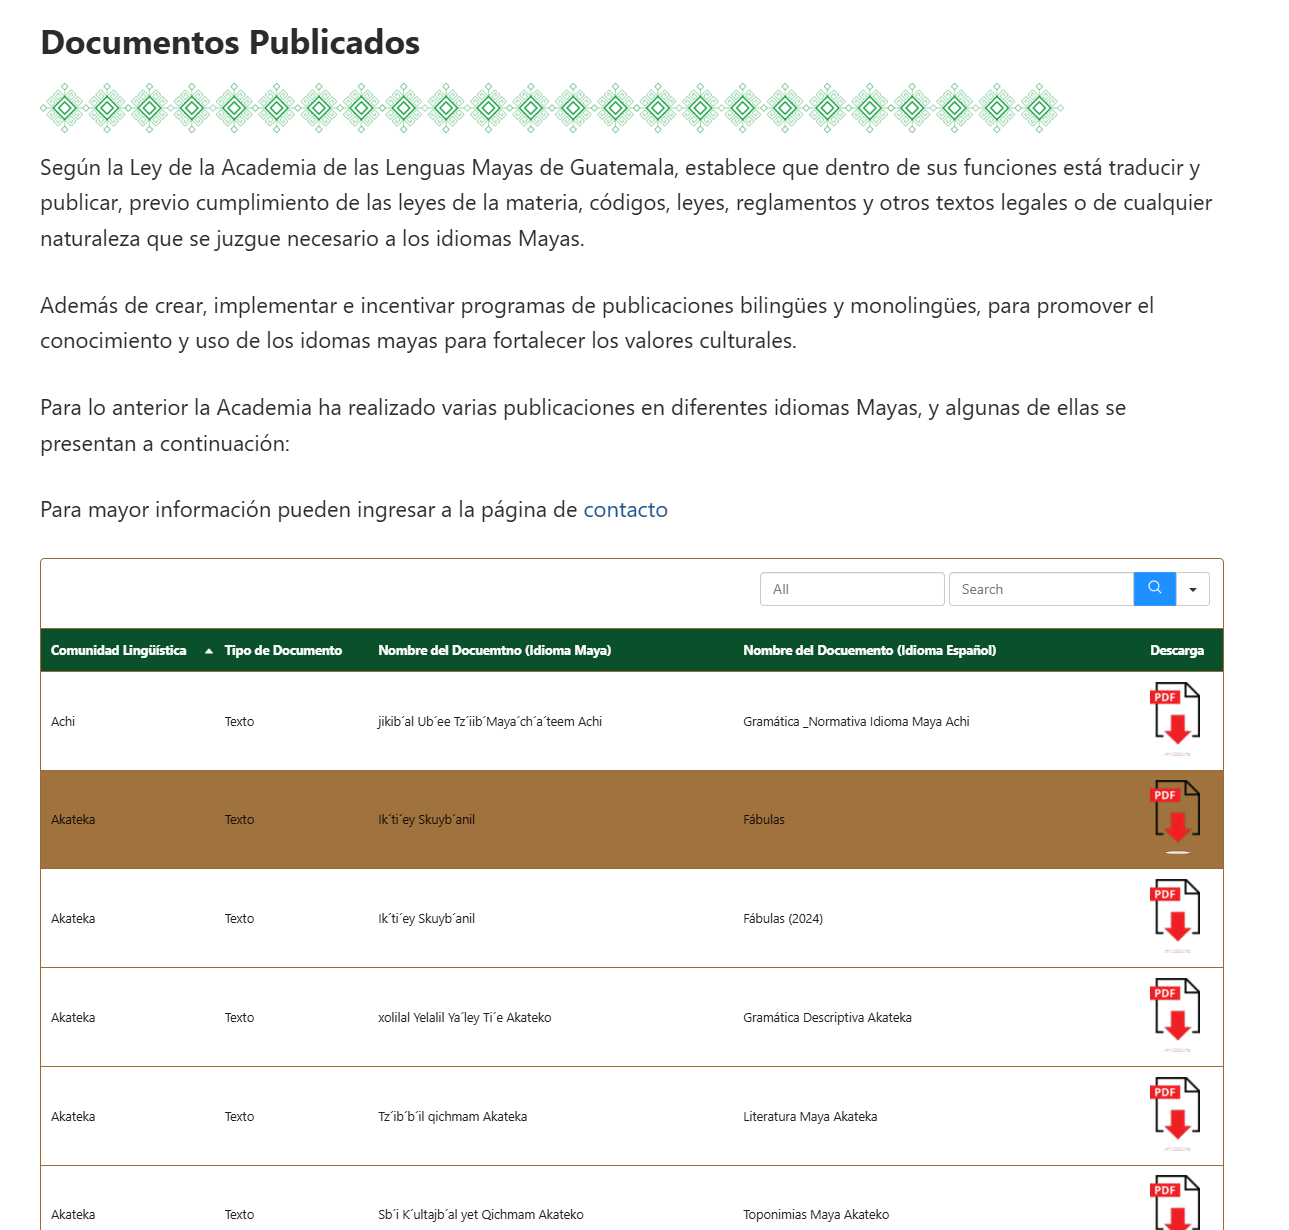
\includegraphics[width=0.95\linewidth]{imagenes/ALMG/web_ALMG.png}
    \caption{Web de la ALMG}
    \label{fig:web_ALMG}
\end{figure}

Por ejemplo, ya en marzo de 2025, tuvieron una actualización de la web en la que eliminaron el 70% de los documentos que tenían alojados, pasando de 200 a 60.
Esta limitación impide que los datos lingüísticos (ejemplos gramaticales, reglas sintácticas, morfología) puedan ser procesados automáticamente por herramientas computacionales, buscadores especializados o sistemas de aprendizaje profundo. La motivación técnica de este trabajo radica, por tanto, en la superación de las barreras impuestas por el reconocimiento óptico de caracteres (OCR) convencional sobre este corpus específico de la ALMG, para generar corpus con morfologías clasificadas para entrenamiento de modelos.
Las gramáticas lingüísticas de estas lenguas presentan una complejidad tipográfica elevada, que incluye tablas anidadas, glosas interlineales y estructuras jerárquicas que los sistemas tradicionales suelen interpretar de manera errónea. Ante este escenario, surge la oportunidad de emplear Modelos de Lenguaje de Gran Tamaño (LLMs), para comprender la arquitectura lógica de estos documentos institucionales y transformarla en datos estructurados bajo el estándar XML.
Este proyecto busca proporcionar una solución eficiente que reduzca la carga de trabajo manual en la digitalización del patrimonio de la ALMG, garantizando que la información sea interoperable, consultable y apta para la generación de documentación científica profesional mediante LaTeX.




\cleardoublepage %salta a nueva página impar
% Aquí va la dedicatoria si la hubiese. Si no, comentar la(s) linea(s) siguientes
\chapter*{Agradecimientos}
\setlength{\leftmargin}{0.5\textwidth}
\setlength{\parsep}{0cm}
\addtolength{\topsep}{0.5cm}

\begin{flushright}
\small\em{
A mi familia por estar ahí en todo momento.\\
A mi pareja por ayudarme en todo lo que puede y más.\\
A mi madre por dedicar su vida a sus hijos.\\
A mi padre por animarme con mi carrera en la ciencia.\\
A mis compañeros del Santander por guiarme y enseñarme cómo desarrollar software. \\
Sin ellos no habría podido hacer este trabajo.
}
\end{flushright}



\cleardoublepage %salta a nueva página impar
% Aquí va la cita célebre si la hubiese. Si no, comentar la(s) linea(s) siguientes
\chapter*{}
%\setlength{\leftmargin}{0.5\textwidth}
%\setlength{\parsep}{0cm}
%\addtolength{\topsep}{0.5cm}
\epigraph{
Pues hemos nacido para colaborar,
al igual que los pies, las manos,
los párpados, las hileras de dientes,
superiores e inferiores. 
Obrar, pues, como adversarios los unos de los otros
es contrario a la naturaleza.
}
{Marco Aurelio (Meditaciones)}
\vspace{4cm}
\epigraph{
    Solo los que se quemaron con el fuego aprendieron a usarlo.
}
{Andrés Pedreño Muñoz\\Cofundador de Torre Juana OST}

\cleardoublepage %salta a nueva página impar

%Con los siguientes comandos se genera el índice, indice de figuras, tablas y listados de código
\tableofcontents
\listoffigures
\listoftables
\lstlistoflistings
